\documentclass[10pt,twocolumn,letterpaper]{article}
%\usepackage[10pt,inchmargins]{sigmin}  %% template from Xi Wang.
\special{papersize=8.5in,11in}
\setlength{\pdfpagewidth}{8.5in}
\setlength{\pdfpageheight}{11in}
\usepackage[noheadfoot,
            left=1in,right=1in,top=1in,bottom=1in,
            columnsep=0.3in
            ]{geometry}
\usepackage[small,compact]{titlesec}
\usepackage[font={small,bf}]{caption}    % added 9/10/13
\usepackage[nolineno,noindent,norules]{lgrind}
\usepackage{tightenum}
\usepackage{float}
\usepackage{xspace}
\usepackage{times,pifont}
\usepackage{mathptmx}
\usepackage{subfig,graphics,graphicx,color}
\usepackage{multirow}
\usepackage{dblfloatfix} %% correctly orders single- and double-col figures
\usepackage{hyphenat}
\usepackage{mathrsfs}
\usepackage{subfig}
\usepackage{amssymb,amsmath,centernot}
\usepackage{lastpage}
\usepackage{flushend}
\usepackage{hhline}
\usepackage{authblk}
%\newcommand{\doi}{XXXXXX}


%%% ================= START of SOSP '13 template ================= 
% \makeatletter
% 
% \def\ftype@copyrightbox{8}
% \def\@copyrightspace{
% \@float{copyrightbox}[b]
% \begin{center}
% \setlength{\unitlength}{1pc}
% \begin{picture}(20,6.0) 
% \put(0,3){\parbox{\columnwidth}{\scriptsize
% 
% %*** SAMPLE. AUTHOR PUT SUPPLIED TEXT HERE ****
% 
% \noindent
% \rule{6.0 cm}{0.2pt}\\
% Permissiondddd to make digital or hard copies of part or all of this work 
% for personal or classroom use is granted without fee provided that
% copies are not made or distributed for profit or commercial advantage 
% and that copies bear this notice and the full citation on the first
% page. Copyrights for third-party components of this work must be
% honored.  For all other uses, contact the Owner/Author. 
% 
% \vspace{\baselineskip}\noindent
% Copyright is held by the Owner/Author(s).\\
% \textit{SOSP'15}.\\
% ACM XXXXXXX.
% 
% \noindent
% http://dx.doi.org/\doi}
% }
% \end{picture}
% \end{center}
% \end@float}
% 
% \def\maketitle{\par
%  \begingroup
%    \def\thefootnote{\fnsymbol{footnote}}
%    \def\@makefnmark{\hbox
%        to 0pt{$^{\@thefnmark}$\hss}}
%      \twocolumn[\@maketitle]
% \@thanks
%  \endgroup
%  \setcounter{footnote}{0}
%  \let\maketitle\relax
%  \let\@maketitle\relax
%  \gdef\@thanks{}\gdef\@author{}\gdef\@title{}\gdef\@subtitle{}\let\thanks\relax
%  \@copyrightspace}
% 
% \makeatother

%%% ================= END of SOSP '13 template ================= 



%\newcommand{\comment}[1]{}
\frenchspacing

%\doublespacing

%%%%%%%%%%%%%%%%%%%%%%%%%%%%
%     macro

\newcommand{\xxx}{\mbox{\textsc{Crane}}\xspace}
\newcommand{\paxos}[0]{\textsc{Paxos}\xspace}
\newcommand{\mytitle}[0]{\textbf {\paxos Made Transparent}}
\newcommand{\mykeywords}[0]{State Machine Replication, Fault Tolerance, Stable Multithreading,
  Software Reliability}

%%%%%%%%%%%%%%%%%%%%%%%%%%%%%%%%%%%%%%%%%%%%%%%%%%%%%%%%%%%%%%%%%
% hyperref stuff

\usepackage[square,comma,numbers,sort]{natbib}
\usepackage{hypernat}
\usepackage{hyperref}

%% fill in pdf info here
\hypersetup{%
colorlinks=false,
pdfborder={0 0 0},
pdftitle={\mytitle},
pdfkeywords={\mykeywords},
bookmarksnumbered,
pdfstartview={FitH},
urlcolor=cyan,
pdfpagelabels=true,
pdfdisplaydoctitle=true,
}%

%\usepackage{breakurl}
%\usepackage[all]{hypcap}
%\renewcommand{\url}{\burl}

%%%%%%%%%%%%%%%%%%%%%%%%%%%%%%%%%%%%%%%%%%%%%%%%%%%%%%%%%%%%
% Some NICE fonts

\newfont{\BIG}{cminch}                             %--- One-inch font
\newfont{\sfbHuge}{cmssbx10 scaled\magstep5}       %-- 25pt sans serif bold
\newfont{\sfbLarger}{cmssbx10 scaled\magstep3}   %-- 12+pt sans serif boldd
\newfont{\sfblarger}{cmssbx10 scaled\magstep2}   %-- 12+pt sans serif bold
\newfont{\sfblarge}{cmssbx10 scaled\magstep1}      %-- 12pt sans serif bold
\newfont{\sfbeleven}{cmssbx10 scaled\magstephalf}  %-- 11pt sans serif bold
\newfont{\sfb}{cmssbx10}                           %-- 10pt sans serif bold
\newfont{\sfeight}{cmss8}                          %-- 8pt sans serif

%%%%%%%%%%%%%%%%%%%%%%%%
%    space tweaking

%\textwidth = 6.5 in
%\textheight = 9.0 in
%\setlength{\topmargin}{-.5in}

%\headheight = 0.0 in
%\headsep = 0.0 in
%\parskip = 0.2in
%\parindent = 0.0in

\renewcommand{\topfraction}{0.95}
\addtolength{\textfloatsep}{-0.1in}
%\addtolength{\floatsep}{0.025in}
\renewcommand\floatpagefraction{.9}
%\renewcommand\bottomfraction{.9}
\renewcommand\textfraction{.1}

\setlength{\parindent}{9pt}

% Rescue
\makeatletter
\def\v#1{{\mbox{\fontfamily{cmtt}\fontsize{\f@size}{\f@size}\selectfont #1}}}

\newcommand{\dmt}[0]{DMT\xspace}
\newcommand{\smt}[0]{StableMT\xspace}
\newcommand{\smr}[0]{SMR\xspace}

\newcommand{\repbox}{\mbox{\textsc{RepBox}}\xspace}
\newcommand{\racepro}[0]{\textsc{RacePro}\xspace}
\newcommand{\criu}[0]{\textsc{CRIU}\xspace}
\newcommand{\tern}[0]{\textsc{Tern}\xspace}
\newcommand{\peregrine}[0]{\textsc{Peregrine}\xspace}
\newcommand{\parrot}[0]{\textsc{Parrot}\xspace}
\newcommand{\grace}[0]{Grace\xspace}
\newcommand{\coredet}[0]{\textsc{CoreDet}\xspace}
\newcommand{\kendo}[0]{Kendo\xspace}
\newcommand{\dthreads}[0]{\textsc{DThreads}\xspace}
\newcommand{\determinator}[0]{Determinator\xspace}
\newcommand{\dos}[0]{dOS\xspace}
\newcommand{\ddos}[0]{DDOS\xspace}
\newcommand{\timealgo}[0]{time bubbling\xspace}
\newcommand{\ldpreload}[0]{LD\_PRELOAD\xspace}

\newcommand{\apache}{\v{Apache}\xspace}
\newcommand{\mongoose}[0]{\v{Mongoose}\xspace}
\newcommand{\ab}{\v{ApacheBench}\xspace}
\newcommand{\clamav}{\v{ClamAV}\xspace}
\newcommand{\upnp}{uPnP\xspace}
\newcommand{\mediatomb}{\v{MediaTomb}\xspace}
\newcommand{\mencoder}{\v{mencoder}\xspace}
\newcommand{\mongodb}{\v{MongoDB}\xspace}
\newcommand{\ssdb}{\v{SSDB}\xspace}
\newcommand{\mysql}{\v{MySQL}\xspace}
\newcommand{\sysbench}{\v{SysBench}\xspace}
\newcommand{\zookeeper}{\v{ZooKeeper}\xspace}


\newcommand{\aget}[0]{\v{aget}\xspace}
\newcommand{\pthread}[0]{\mbox{Pthreads}\xspace}
\newcommand{\openldap}[0]{{OpenLDAP}\xspace}
\newcommand{\redis}[0]{{Redis}\xspace}
\newcommand{\bdb}[0]{{Berkeley DB}\xspace}
\newcommand{\vtune}[0]{\v{VTune}\xspace}
\newcommand{\http}[0]{\mbox{HTTP}\xspace}

% In short.
\newcommand{\eg}{{e.g.}}
\newcommand{\ie}{{i.e.}}
\newcommand{\etc}{{etc}}
\newcommand{\para}[1]{\vspace{.00in}\noindent{\bf #1}}
\newcommand{\wrt}{{w.r.t. }}
\newcommand{\cf}{{cf. }}

% Synch and network operations.
\newcommand{\mutexlock}[0]{\v{pthread\_mutex\_lock()}\xspace}
\newcommand{\connect}[0]{\v{connect()}\xspace}
\newcommand{\send}[0]{\v{send()}\xspace}
\newcommand{\close}[0]{\v{close()}\xspace}
\newcommand{\recv}[0]{\v{recv()}\xspace}
\newcommand{\select}[0]{\v{select()}\xspace}
\newcommand{\poll}[0]{\v{poll()}\xspace}
\newcommand{\epollwait}[0]{\v{epoll\_wait()}\xspace}
\newcommand{\accept}[0]{\v{accept()}\xspace}

% Parrot primitives.
\newcommand{\getturn}[0]{\v{get\_turn()}\xspace}
\newcommand{\putturn}[0]{\v{put\_turn()}\xspace}
\newcommand{\wait}[0]{\v{wait()}\xspace}
\newcommand{\signal}[0]{\v{signal()}\xspace}

% Evaluation stats.
\newcommand{\github}[0]{\url{anonymous}}
\newcommand{\ntype}[0]{three\xspace}
\newcommand{\nprog}[0]{four\xspace}
\newcommand{\overhead}[0]{10.9\%\xspace}
\newcommand{\dmtspeedup}[0]{10.5\%\xspace}
\newcommand{\proxyoverhead}[0]{1.7\%\xspace}
\newcommand{\recovertime}[0]{0.82s\xspace}
\newcommand{\mencoderspeedup}{\v{49\%}\xspace}

\def\LGfsize{\footnotesize}
%\pagestyle{empty}

\begin{document}

% Hack for: Package caption Error: No float type 'copyrightbox' defined.
%\newcounter{copyrightbox}

\date{}

\title{\mytitle}

\author[+]{\hspace{0 mm}\fontsize{10}{10}\selectfont Authors}
\maketitle
%\thispagestyle{empty}

\begin{sloppypar}
\begin{abstract}

Nevertheless, previous approaches do not target the availability at the application 
level, but rather at the VM level, therefore service-continuity cannot be 
guaranteed in case of application failure.

This paper presents \xxx, an SMR system for KVM based virtualized machines, 
which efficiently replicates programs running in the virtual machines. 
\xxx achieves distributed consensus at the networking level of QEMU. 
Evaluation on five widely used server programs (e.g., \mysql and \redis) shows 
that \xxx is easy to use and has low overhead.

\end{abstract}
\end{sloppypar}

% \begin{sloppypar}
%% %\category{D.2.5}{Software Engineering}{Testing and Debugging}
%% \category{D.4.5}{Operating Systems}{Threads, Reliability}
%% \category{D.2.4}{Software Engineering}{Software/Program Verification}
%% \terms{Algorithms, Design, Reliability, Performance}
%% \keywords{\mykeywords}

%% \vskip 2mm
%% \noindent {\small \bf Categories and Subject Descriptors:} \vskip -.2mm
%% \noindent
%% {\footnotesize D.4.5~[{\bf Operating Systems}]: {Threads, Reliability}\\
%% D.2.4~[{\bf Software Engineering}]: {Software/Program Verification};}
%% \vskip 1mm
%% \noindent {\small \bf General Terms:} \vskip -.2mm
%% \noindent
%% {\footnotesize Algorithms, Design, Reliability, Performance}
%% \vskip 1mm
%% \noindent {\small \bf Keywords:} \vskip -.2mm
%% \noindent
%% {\footnotesize \mykeywords}

% \vskip 2mm
% \noindent {\small \bf Categories and Subject Descriptors:}
% {\small D.4.5~[{\bf Operating Systems}]: {Threads, Reliability};
%   D.2.4~[{\bf Software Engineering}]: {Software/Program Verification};}
% \vskip .1mm
% \noindent {\small \bf General Terms:} {\small Algorithms, Design,
%   Reliability, Performance}
% \vskip .1mm
% \noindent {\small \bf Keywords:} {\small \mykeywords}
% 
% \end{sloppypar}

%%%%%%%%%%%%%%%%%%%%%%%%%%%%%%%%%%%
% Add page number.
\setcounter{page}{1}
\pagenumbering{arabic}

\thispagestyle{plain}
\pagestyle{plain}
\setlength{\footskip}{20pt}
%%%%%%%%%%%%%%%%%%%%%%%%%%%%%%%%%%%

\begin{sloppypar}

\section{Introduction} \label{sec:intro}

% P1: virtualization is good
By allowing multiple servers to be consolidated on a small number of physical hosts 
and simplifying provisioning, virtualization is widely used in computing environments 
of various kinds and scales.

% P2: However, previous approaches still fail to efficiently and reliably provide fault-tolerance in virtualized environment
% checkpoint-recovery based replication suffers from two problems
% 1. performance degradation due to the large amount of state that needs to be synchronized between the primary and the backup machines
% 2. significant VM downtimes
% 3. network delay
Nevertheless, server consolidation exacerbates the consequence of unexpected host failures. 
When VMs are consolidated, failure of a single host may bring down mutiple VMs on the host 
and all applications running thereon, resulting in an unacceptable aggregate loss. 
To accommdote virtual machines with high availability, various approaches have been 
proposed to replicate VMs between hosts continuously throughout VM's execution, but 
they are still unable to ensure fault-tolerance in virtualized environments efficiently 
and reliably. One typical technique is checkpoint-recovery based replication of virtual 
machines. It captures the entire execution state of the running VM at relatively 
high frequency so that changes can be reflected to the backup machine nearly instantly. 
One disadvantage of the checkpoint-recovery based replication is the amount of data that 
needs to be copied from the primary to the backup, which can, in some cases, seriously 
affect the performance. Apart from that, VM downtimes incurred by the checkpoint mechanism 
can be significant.

% P3: derterministic replay is the other approach which can address some of the drawbacks of checkpoint-recovery based replication
% single point of failure
% slow for multi-processor

% To answer Heming's question: old leader and new leader get to an inconsistent state
% After recovery, the old leader should be started in the state as the new leader before participating

% 6.824 2016 mit
% What if the network between primary/backup fails?
%  -Primary is still running
%  -Backup becomes a new primary
%  -Two primaries at the same time!
% one can avoid split brain using a single "master"
% master computer decides whether replica A or replica B is the primary
%   there's just one master, so it never disagrees with itself
% clients talk to the master
% this is probably what VMware FT does (atomic test-and-set in shared disk)
% but what if the master fails?
%   it's a "single point of failure" -- not so good
% VMware FT shared disk atomic test-and-set was (apparently) not replicated

% In the non-shared-disk configuration, there may be no shared storage to use for dealing with a split-brain situation.
% In this case, the system could use some other external tiebreaker, such as a third-party server that both servers can talk to.
% If the servers are part of a cluster, the system could alternatively use a majority algorithm based on cluster membership.

On the other hand, derterministic replay is an attractive technique which can address the 
aforementioned drawbacks of checkpoint-recovery based replication: primary and backup execute 
the same sequence of instructions, with non-deterministic events injected exactly at the same 
point into both replicas. However, in the existing works, in order to avoid split brain, 
derterministic replay has to suffer from "single point of failure".

Fortunately, \paxos, a majorty vote algorithm, can be used to prevent the split-brain scenarios 
across the cluster. Moreover,  \paxos provides another great benefit: it ensures the same sequence 
of input requests for replicas. But \paxos is notoriously slow because each decision takes at least 
three message delays between when a replica proposes a command and when some replica learns which 
command has been chosen.

Luckily, Remote Direct Memory Access (RDMA)-capable networks have dropped in price and made 
substantial inroads into datacenters. It allows one computer to directly access the memory of 
a remote computer without involving the operating system at any host. This enables zero-copy 
transfers, reducing latency and CPU overhead.

The remainder of the paper is organized as follows.

% \section{Background} \label{sec:background}

\subsection{KVM} \label{sec:kvm}

KVM is a more recent hypervisor which embeds virtualization capabilities 
in Linux kernel using x86 hardware virtualization extensions~\cite{kivity2007kvm}. 
It is a full virtualization solution, where guests are run unmodified in VMs. It 
consists of two modules, namely, kvm.ko module and an architecture dependent 
kvm-amd.ko or kvm-intel.ko module. Under KVM, each VM is spawned as a regular linux 
process named KVM and scheduled by the default linux scheduler. 

For using shared I/O hardware, these VMs interact with Qemu emulator in host user 
space which provides emulated I/O devices for virtual machines. For instance, in 
the case of network related applications, Qemu provides emulated Network Interface 
Card (NIC) to VMs and interacts with tun-tap device on the other side. The tap device 
is connected to physical NIC through a software bridge.

Figure 1 shows the typical KVM architecture, with reference to a network related
application. 

As depicted in the picture, when a packet arrives at physical NIC,
interrupts generated by NIC are handled by the physical device driver. The device
driver forwards the packet to software bridge. The bridge, then pushes the packet
to the tap device of the corresponding VM. The tap device is a virtual network
device that sends a signal to KVM module. KVM module in turn, generates a virtual
interrupt to the user space Qemu of the target VM. Qemu then copies the packet from
tap device and generates the interrupt for the guest OS emulating the virtual NIC.
Again, the physical device driver in the guest OS handles the packet transfer to
the VM’s address space. A major advantage of the KVM architecture is the full
availability of user-space tools in the QEMU process, such as threading, libraries
and so on.

\begin{figure}[t]
% \vspace{.20in}
\centering
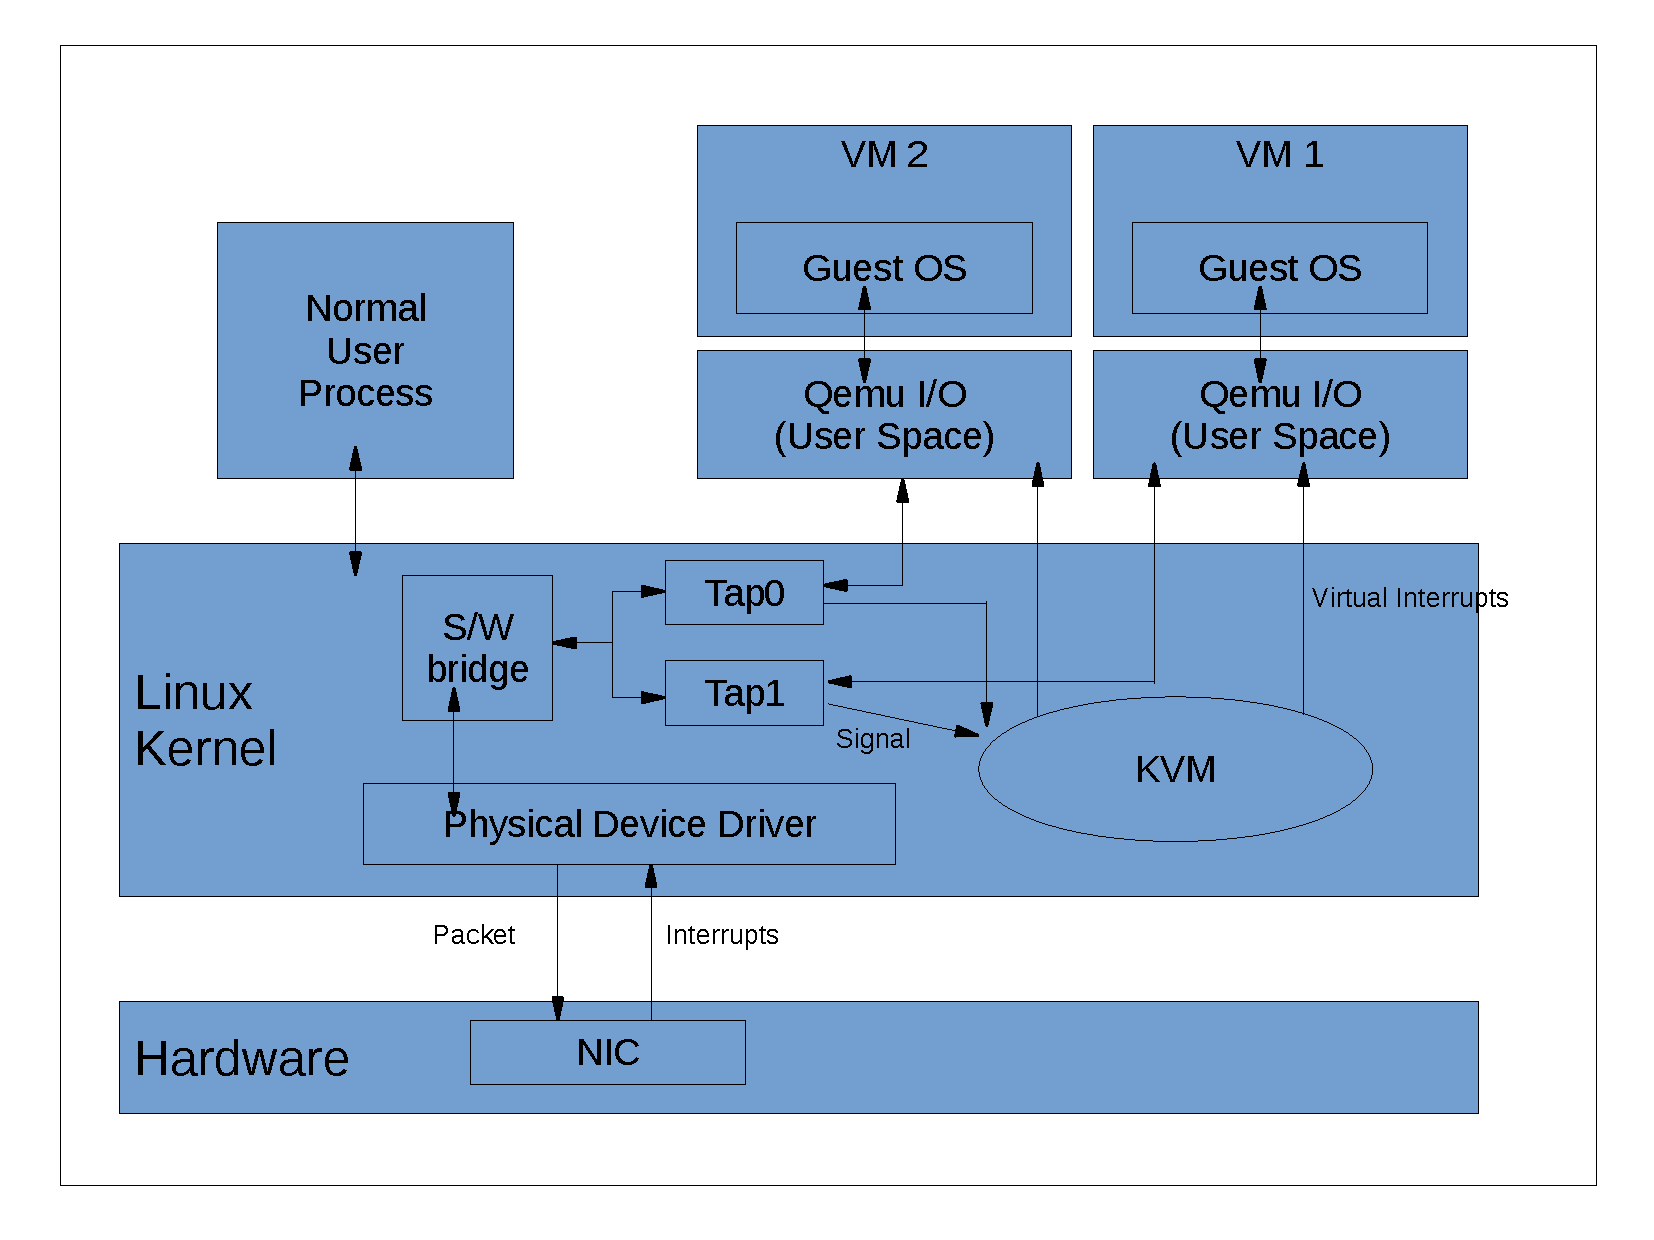
\includegraphics[width=.47\textwidth]{figures/kvm}
\vspace{-.2in}
\caption{{\em KVM Architecture.}} \label{fig:kvm}
\vspace{.05in}
\end{figure}

\subsection{FALCON} \label{sec:falcon}

\smrsystem's deployment model is similar to a typical \smr's. In a \smrsystem-replicated 
system, a set of $2f+1$ machines (nodes) are set up in a InfiniBand cluster. Once the 
\smrsystem system starts, one node becomes the \emph{primary} node which proposes the order of 
requests to execute, and the others become backup nodes which follow the primary’s 
proposals. An arbitrary number of clients in LAN or WAN send network requests to the 
primary and get responses. If failures occur, the nodes run a leader election to elect 
a new leader and continue.

On receiving a client network request, it invokes a RDMA-based consensus process on this 
request to enforce that all replicas see the same sequence of input requests. This process 
has three steps. In the first step, the leader assigns a global, monotonically increasing 
viewstamp to this request, stores this request into an entry that is appended to the consensus 
log, and does a forced write to the local disk. The second step is to replicate the log entry 
on remote servers using a one-sided RDMA Write operation. Usually when the RDMA NIC (RNIC) 
completes the network steps associated with the RDMA operation, it pushes a completion event 
to the queue pair's associated completion queue (CQ) via a DMA write. Using completion events 
adds extra overhead. Since \paxos could help handle the reliability issues, \smrsystem takes 
advantage of unsignaled RDMA write operations, i.e., a completion event will not be pushed for 
these operations, to reduce that overhead. In the last step, the leader thread waits for 
acknowledgments from a majority of nodes.

In addition to the distributed consensus protocol for coordinating the sequence of input requests, 
\smrsystem also runs an output checking protocol which compares each replica's network outputs 
occasionally to detect the divergence of execution states.

% \input{overview}
% \input{interface}
% \input{consensus}
% \section{Implementation} \label{sec:impl}

% SMR. Paxos.

% DMT.

% Checkpoint.
% \input{discussion}
% % \newpage
\section{Evaluation} \label{sec:eval}

% We evaluated an anti-virus scanning server that a b c d e f.

\begin{table}[b]
\footnotesize
\centering
\vspace{-.05in}
\begin{tabular}{lrrr}
{\bf Approach} & {\bf Resp time (s)} & {\bf Overhead (\%)} \\
\hline\\[-2.3ex]
Native execution                       & 1.14  &        \\
\xxx framework only                       & 3.03   & 0     \\
\xxx with Helgrind                                   & 20.96 & 0     \\
\xxx with Helgrind and XX                       & 23.76 & 0       \\
Helgrind only                       & 23.76 & 0       \\
\end{tabular}
\vspace{-.05in}
\caption{{\em Percentage of inserted time bubbles among all consensus 
requests.}} 
\label{tab:bubble-percentage}
\end{table}

We evaluated \xxx on \clamav, an anti-virus scanning server that scans files 
parallely and deletes malicious ones. Our evaluation was done on a set of three 
Linux 3.2.14 machines within a 1Gbps bandwidth LAN, and each machine has 2.80 
GHz dual-socket hex-core Intel Xeon with 24 hyper-threading cores and 64GB 
memory. we used \clamav's own client utility \v{clamdscan} to request the server 
to parallely scan \clamav's own source code and installation directories. we 
measured each workload's response time because it has direct impact on users.


% \section{Related Work} \label{sec:related}

\para{Cluster Management System.} Cluster management 
systems~\cite{borg:eurosys15,mesos:nsdi11,tupperware,yarn:socc13,
autopilot:sosp07,quincy:sosp09,apollo:osdi14,fuxi:vldb14} are widespread 
because they can transparently support many diverse applications (\eg, 
Hadoop~\cite{hadoop}, Dryad~\cite{dryad}, and key-value stores~\cite{redis}). 
These existing systems mainly focus on high availability for themselves by 
replicating important components (\eg, controllers) within these systems, or 
focus on fault-recovery of applications~\cite{fuxi:vldb14}. To the best of our 
knowledge, no existing system provides efficient and general high-availability 
service to applications. Although \xxx's current design leverages an existing 
system Mesos~\cite{mesos:nsdi11}, its general \paxos protocol design can also 
be integrated in other systems.

\para{State machine replication (SMR).}  SMR is a powerful, but 
complex fault-tolerance technique. The literature has developeed a rich set of
\paxos 
algorithms~\cite{paxos:practical,paxos,paxos:simple,paxos:complex,epaxos:sosp13}
and implementations~\cite{paxos:live,paxos:practical,chubby:osdi}. \paxos is 
notoriously difficult to be fast and scalable~\cite{ellis:thesis}. To improve 
speed and scalability, various advanced replication models have been 
developed~\cite{epaxos:sosp13,mencius:osdi08,scatter:sosp11,manos:hotdep10}. 
Since consensus protocols play a core role in 
datacenters~\cite{matei:hotcloud11, mesos:nsdi11, datacenter:os} and 
distributed 
systems~\cite{spanner:osdi12,mencius:osdi08}, a variety of study have been 
conducted to improve different aspects of consensus protocols, including 
performance~\cite{epaxos:sosp13,paxos:fast,dare:hpdc15}, 
understandability~\cite{raft:usenix14,paxos}, and verifiable reliability 
rules~\cite{modist:nsdi09,demeter:sosp11}. Although \xxx tightly integrates 
RDMA features in \paxos, its implementation mostly complies with a popular, 
practical approach~\cite{paxos:practical} for reliability. Other \paxos 
approaches can also be leveraged in \xxx.

\para{RDMA techniques.} RDMA techniques have been implemented in various 
architectures, including Infiniband~\cite{infiniband}, RoCE~\cite{roce}, and 
iWRAP~\cite{iwrap}. RDMA have been leveraged in many systems to improve 
application-specific latency and throughput, including high performance 
computing~\cite{openmpi}, key-value 
stores~\cite{pilaf:usenix14,herd:sigcomm14,farm:nsdi14,memcached:rdma}, 
transactional processing systems~\cite{drtm:sosp15,farm:sosp15}, and file 
systems~\cite{gibson:nfs}. These systems are largely complementary to \xxx.
% It 
% will be interesting to investigate whether \xxx can improve the availability 
% for 
% both the client and server for some of these advanced systems within a 
% datacenter, and we leave it for future work.
% \section{Conclusion} \label{sec:conclusion}

We have presented \xxx, an efficient, transparent dynamic program analysis 
framework. It leverages \smr and \dmt to consturct multiple equavalent 
executions in replicas, so that actual executions and analyses can be fully 
decoupled. Evaluation shows that \xxx can transparently run analyses on 
replicas with reasonable overhead. Furthermore, analyses and \xxx can be 
mutually beneficial. \xxx has the potential to promote the deployments of 
powerful analyses in applications' production runs.
% \section*{Acknowledgments}
% TBD.
We thank Jian Ouyang (our shepherd) and anonymous reviewers for
their many helpful comments.
This work was supported in part by AFRL FA8650-11-C-7190 and FA8750-10-2-0253;
ONR N00014-12-1-0166; NSF CCF-1162021, CNS-1054906;
an NSF CAREER award; an AFOSR YIP award; and a Sloan Research Fellowship.


\end{sloppypar}

% uncomment to tweak with bib spacing
%\setlength\bibsep{2.25pt}
{
%\small
 \bibliographystyle{abbrvnat}
 \bibliography{bib/biblio}
}

\end{document}
